\documentclass{source/Report}

\major{电子科学与技术}
\name{朱炳昊}
\title{NA Project}
\stuid{3220105656}
\college{信息与电子工程学院}
\date{\today}
\lab{西2-213}
\course{数值分析方法}
\instructor{余官定}
\grades{}
\expname{稀疏矩阵特征值}
\exptype{大作业报告}
\partner{无}

\begin{document}
    \makecover
    \makeheader
    \tableofcontents
    \newpage
    \section{背景介绍}
    在实际的工程和科学应用中,我们经常会遇到大规模的数据集,这些数据通常以矩阵的形式呈现。许多情况下,这些矩阵主要由零元素构成,只有少部分非零元素,我们称这种矩阵为“稀疏矩阵”。在诸如社交网络分析、图像处理、自然语言处理、有限元分析、物理学模拟等多个领域,我们都会遇到稀疏矩阵。由于这些领域的数据通常具有高维度,但又由于各种原因,矩阵中的数据元素只有极小一部分是非零的,因此,如何处理和利用这些稀疏矩阵变得非常重要。

    作为一名正在学习数值分析方法课程的学生,我对这个问题有着浓厚的兴趣。我知道,计算和理解稀疏矩阵的特征值是一个具有挑战性的问题。然而,存在一些专门的数值计算方法,如Power Method、QR 算法和 Arnoldi迭代算法,可以帮助我们解决这个问题。

    在本次期末大作业中,我打算深入研究这些算法,并将它们应用在普通矩阵和高维稀疏矩阵上,比较他们在不同类型矩阵上的性能。我相信,通过这项研究,我将能够更深入地理解稀疏矩阵的重要性,以及特征值计算方法的应用。
    \section{设计思路}
    \subsection{设计目的}
    本研究的主要目的是探索和理解数值计算方法在处理稀疏矩阵特征值问题上的应用和性能表现。具体来说,设计目标可分为以下几点:

    (1)深入理解Power Method、QR算法和Arnoldi迭代算法的工作原理和应用场景,以及如何将它们应用于稀疏矩阵的特征值计算。

    (2)比较这些算法在普通矩阵和高维稀疏矩阵上的性能表现,包括计算速度、精度和稳定性等方面。

    (3)深入理解稀疏矩阵在不同领域的应用,以及特征值计算在这些应用中的重要性。

    (4)建立一个能够处理大规模稀疏矩阵特征值问题的计算模型,以展示这些数值计算方法在实际工程和科学应用中的效用。

    通过完成这些目标,我们希望能够为稀疏矩阵特征值的计算提供一种有效的数值计算工具,同时也为理解和应用稀疏矩阵提供一种新的视角和理论支持。
    \subsection{设计流程}
    \begin{itemize}
      \item \textbf{Import necessary libraries:} 首先,我们需要导入开发过程中需要用到的库。
      \item \textbf{Define functions:} 接着,我们定义了一些数学计算函数,包括'sparse\_sym\_matrix'、'power\_method'、'qr\_iteration'、'arnoldi\_iteration1'和'arnoldi\_iteration2'。这些函数分别用于生成稀疏矩阵、实现幂法、QR迭代法和Arnoldi迭代法。
      \item \textbf{Define MainWindow class:} 然后,我们定义了主窗口类'MainWindow',该类主要用于构建用户界面和处理用户操作。
      \item \textbf{Define methods in MainWindow class:} 在'MainWindow'类中,我们定义了一些方法,包括'run\_code'和'open\_readme'。'run\_code'方法用于获取用户输入,调用相应的函数执行计算,然后显示结果。'open\_readme'方法用于打开GitHub上的说明文档。
      \item \textbf{Create QApplication object and MainWindow object:} 最后,我们创建了'QApplication'对象和'MainWindow'对象,并显示GUI窗口。
    \end{itemize}
    
    \subsection{设计环境}
    运行环境为 Python 3.11.5,以下为运行python文件所需调用的库:
    \begin{itemize}
      \item \textbf{numpy:} Python科学计算的核心库,提供了高性能的多维数组对象及相关工具。
      \item \textbf{scipy:} 基于numpy的一种高级计算库,提供了许多有用的数学算法和函数。
      \item \textbf{PyQt5:} Python编写的GUI框架,用于创建桌面应用程序。
      \item \textbf{sys:} Python内置库,提供了访问与Python解释器紧密相关的变量和函数的途径。
      \item \textbf{webbrowser:} Python内置库,提供了一个简单的接口,用于在Web浏览器中显示文档或打开URL。
    \end{itemize}
    
    \section{算法描述}
        

    \section{应用展示}

    \section{时间复杂度分析}

    \section{使用说明}

    \section{总结与展望}
    \begin{algorithm}
        \caption{Algorithm 1 Arnoldi Iteration}
        \begin{algorithmic}[1]
        \State choose $b_1$ arbitrarily, then $q_1 = b_1/\|b_1\|$
        \For{$m = 1,2,\dots,k$}
          \For{$j = 1,2,\dots,m$}
            \State $v_j = q_j - h_jv_j$
          \EndFor
          \State $h_{m+1,m} = \|v_{m+1}\|$
          \State $q_{m+1} = v_{m+1}/h_{m+1,m}$
        \EndFor
        \end{algorithmic}
        \end{algorithm}
        
        
        % \begin{table}[H]
        %     \centering
        %     \caption{雅可比迭代结果-4.1}
        %     \begin{tabular}{cccc}
        %     \toprule
        %     $n$ & $x_1^{(n)}$ & $x_2^{(n)}$ & $x_3^{(n)}$ \\
        %     \midrule
        %     0 & 1.25000000 & -1.33333333 & 0.20000000 \\
        %     1 & 1.63333333 & -0.85555556 & -0.11111111 \\
        %     2 & 1.43611111 & -0.81759259 & -0.04740741 \\
        %     \bottomrule
        %     \end{tabular}
        % \end{table}\par
    
    
        % \lstinputlisting[
        %     language = Python,
        %     title = {最小二乘法线性拟合代码}
        % ]{code/linear_ap.py}\par
        

%             \begin{lstlisting}[language = Verilog, title = {代码块测试(直接插入)}]
% module dffre (
%     d, en, r, clk, q
% );
%     parameter n = 1;
%     input en,r,clk;
%     input [n-1:0] d;
%     output [n-1:0] q;
%     reg [n-1:0] q;
%     always @(posedge clk) begin
%         if(r) q = {n{1'b0}};
%         else if(en) q = d;
%             else q = q;
%     end
% endmodule
%             \end{lstlisting}

%             \begin{figure}[H]
%                 \centering
%                 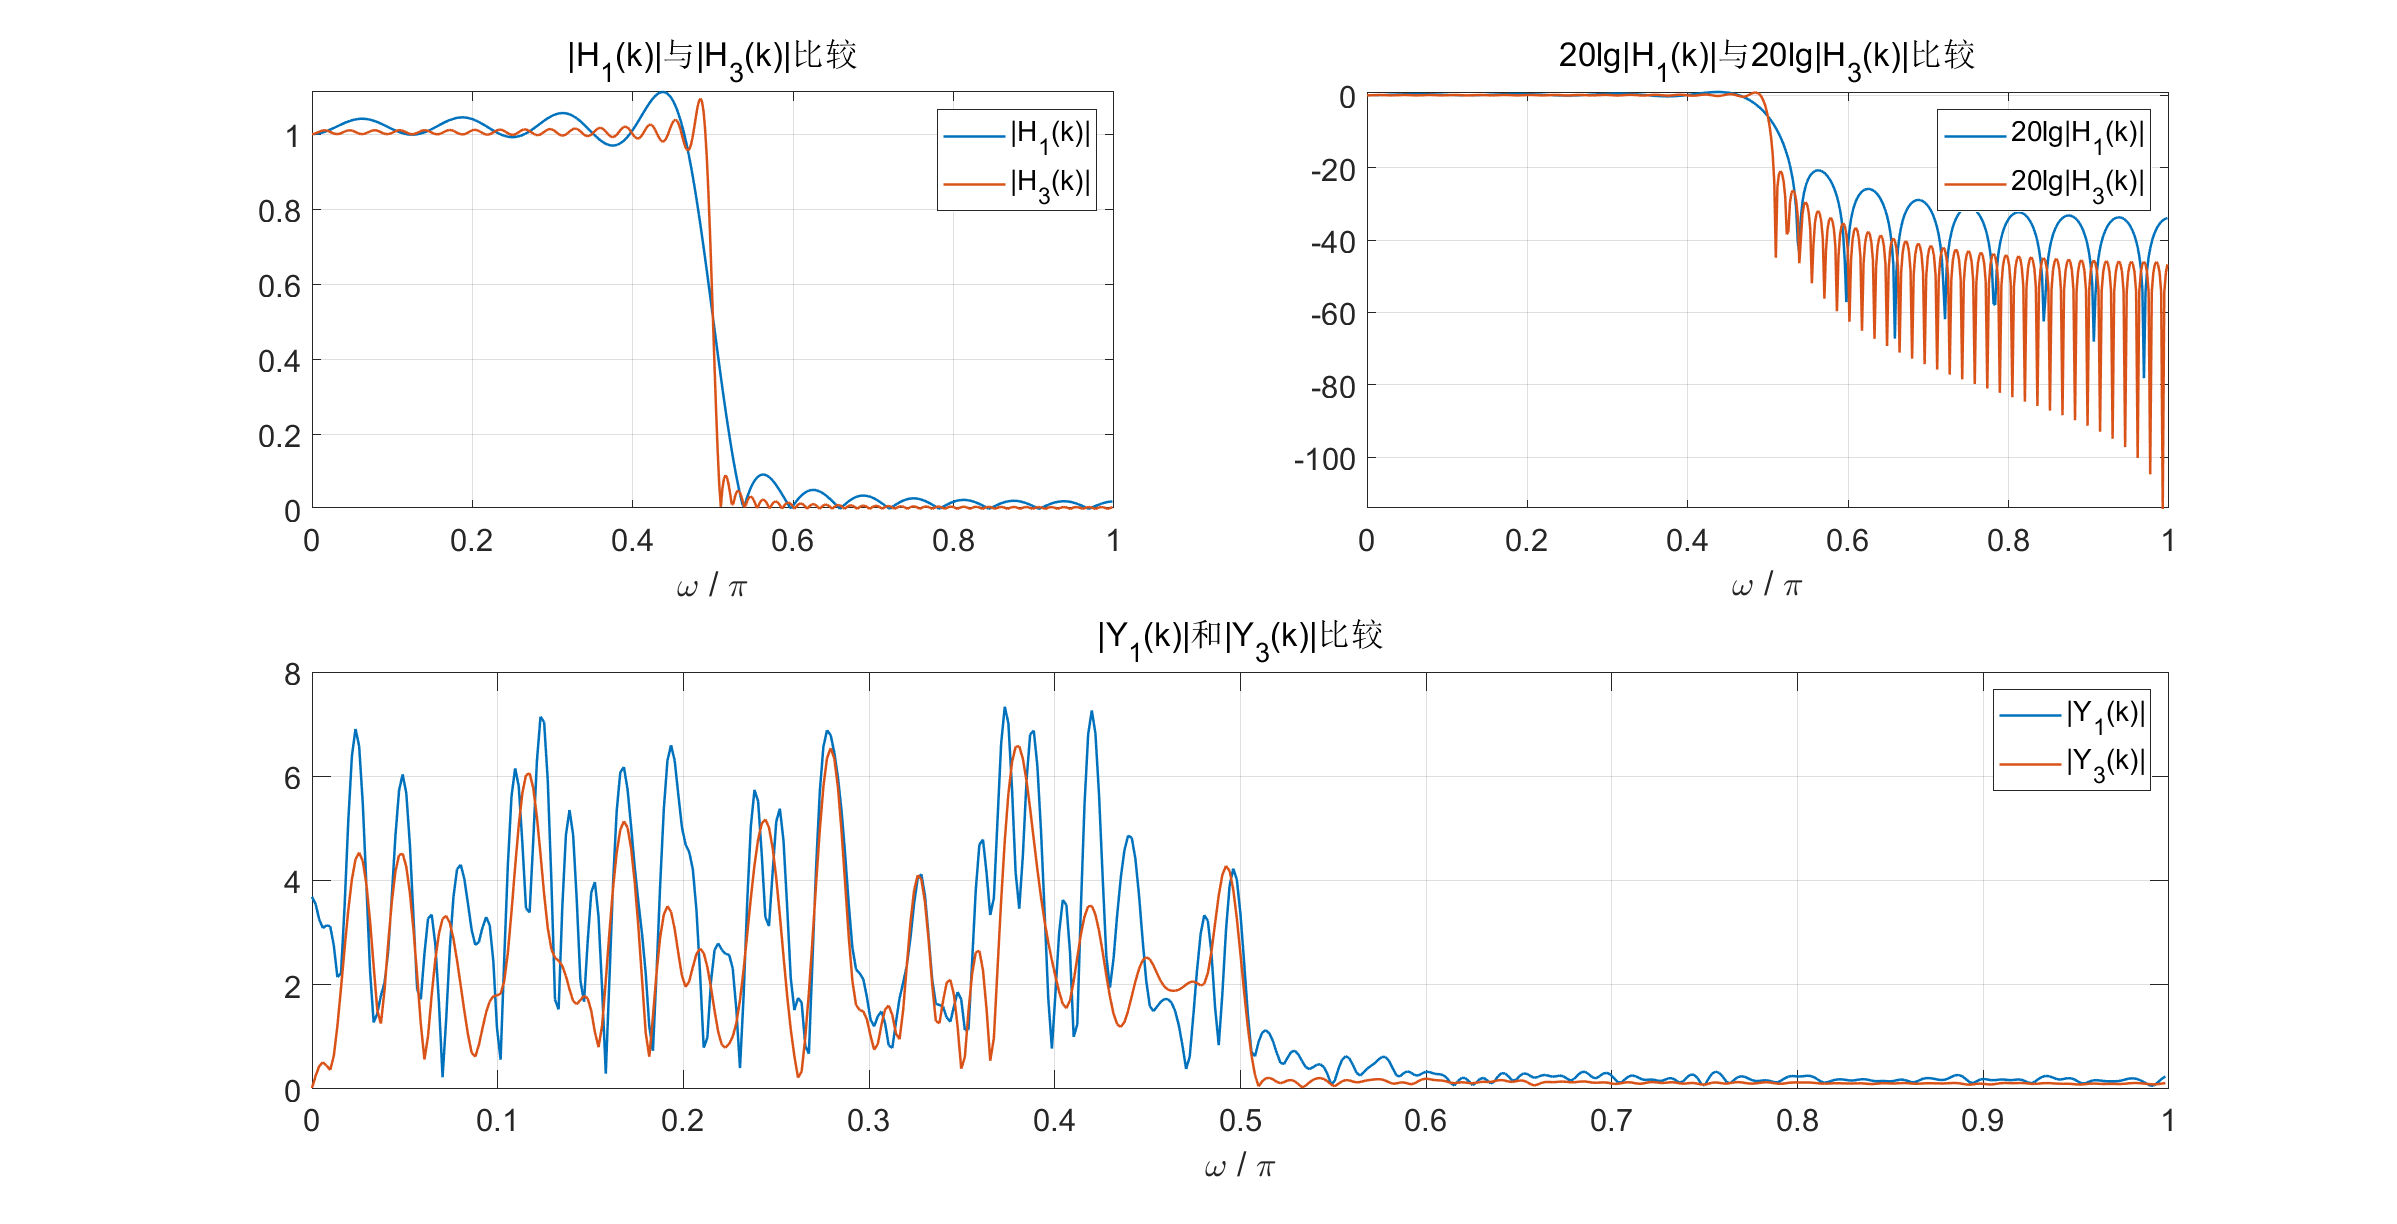
\includegraphics[width = 1\textwidth]{pic1}
%                 \caption{图片测试}
%             \end{figure}


    % \section{}
    %         \subsection{}
    %         1\footnote{测试}2
    %         \begin{table}[H]
    %             \centering
    %             \caption{表格测试}
    %             \begin{tabular}{|c|c|c|c|c|c|c|c|c|}
    %             \hline
    %             state                 & ld & st & addr{[}31:11{]} == tag & valid & dirty & l2\_ack & write\_done & nextstate                   \\ \hline
    %             \multirow{4}{*}{Idle} & 0  & 0  & -                      & -     & -     & -       & -           & Idle                        \\ \cline{2-9} 
    %                                 & 0  & 1  & -                      & -     &       & -       & -           & \multirow{3}{*}{CompareTag} \\ \cline{2-8}
    %                                 & 1  & 0  & -                      & -     &       & -       & -           &                             \\ \cline{2-8}
    %                                 & 1  & 1  & -                      & -     &       & -       & -           &                             \\ \hline
    %         \end{tabular}
    %         \end{table}
\end{document}